
%%%% CAPÍTULO 1 - INTRODUÇÃO
%%
%% Deve apresentar uma visão global da pesquisa, 
%% incluindo: breve histórico, importância e
%% justificativa da escolha do tema, delimitações
%% do assunto, formulação de hipóteses e objetivos
%% da pesquisa e estrutura do trabalho.

% Perguntas que podem guiar a introdução - não necessariamente irá ter a resposta para tudo, isso depende da área.
% 1 - Qual é o contexto em que seu trabalho está inserido?
% 2 - Qual é o problema que motiva a existência deste trabalho?
% 3 - Qual é a visão geral da literatura sobre o problema e como é tratado
% 4 - Por que a solução na literatura não é o suficiente para ?
% 5 - Como seu trabalho trata o problema ?
% 6 - como seu trabalho foi avaliado para comprovar que tratou adequadamente o problema?
% 7 - De forma geral quais foram os resultados ?
% 8 - Quais foram as contribuições do seu trabalho?
% 9 -  Como o restante da Dissertação ou Tese está organizada ?


\chapter{Introdução}
\label{cap:introducao}

Nas anestesias raquidianas os anestesistas dependem do seu sentimento tátil durante a inserção da agulha no paciente para a correta identificação do local de aplicação do líquido anestésico. O local de aplicação da raquidiana é conhecidos como espaço subaracnóideo \cite{Miller2009}). Para que o anestesista reconheça a chegada da agulha neste local ele precisa reconhecer os tecidos ultrapassados por ela. As anestesias possuem técnicas específicas para identificação dos seus espaços de aplicação. Para que os médicos dominem a técnica da anestesia raquidiana é estimado que são necessários 44 ± 6 repetições de execução deste tipo de procedimento. A confirmação de que o local adequado foi atingido na anestesia raquidiana é feita através da observação do vazamento, através da agulha de punção, do liquido cérebro espinhal ou cefalorraquidiano (\textit{líquor}). As Figuras~\ref{fig:puncaoLombar} e ~\ref{fig:gotejamentoLiquor}  ilustram dois momentos importantes da anestesia raquidiana retirados de um video. Na Figura~\ref{fig:puncaoLombar} é mostrado o momento de inserção da agulha para punção lombar e na Figura~\ref{fig:gotejamentoLiquor} é mostrado o vazamento, através da agulha de punção, do (\textit{líquor}), o que acontece alguns segundos após a agulha estar corretamente posicionada no espaço subaracnóideo. Neste tipo de anestesia é usada uma agulha de menor diâmetro do que a agulha utilizada na anestesia epidural \cite{Miller2009}. O ultrassom é uma ferramenta eficiente para auxilio na determinação do espaço onde a agulha precisa ser inserida \cite{Helayel2010}, mas o uso deste tipo de equipamento não é uma realidade em muitos centros do Brasil \cite{Hamaji2016}. O uso deste equipamento, portanto não faz parte do treinamento de muitas faculdades de medicina para anestesias raquidianas. Este treinamento é feito através da palpação da crista ilíaca do paciente.

\begin{figure}[!ht]
   \centering
   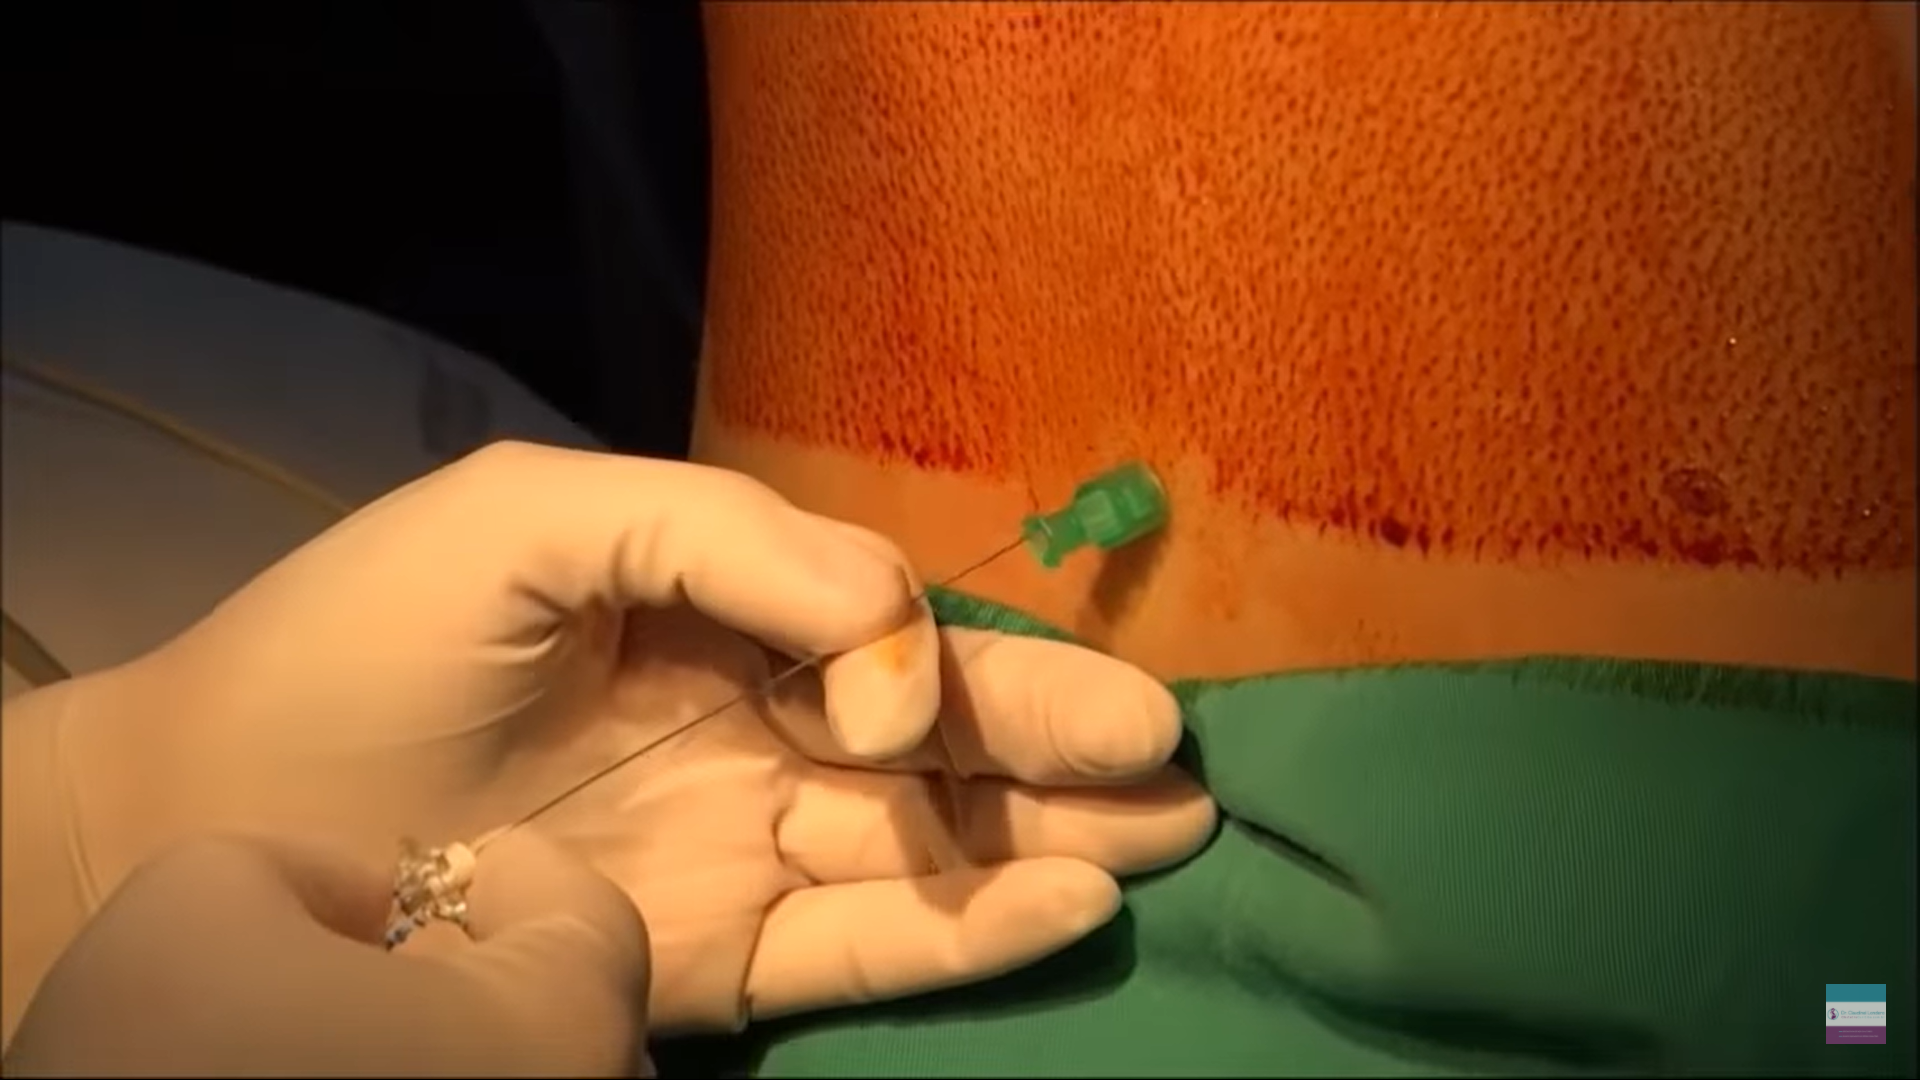
\includegraphics[width=0.6\linewidth]{capitulos/figuras/2.PuncaoLombar.png}
   \caption{Punção lombar com agulha de raquianestesia  \cite{Londero2018}.}
   \label{fig:puncaoLombar}
\end{figure}

\begin{figure}[!ht]
   \centering
   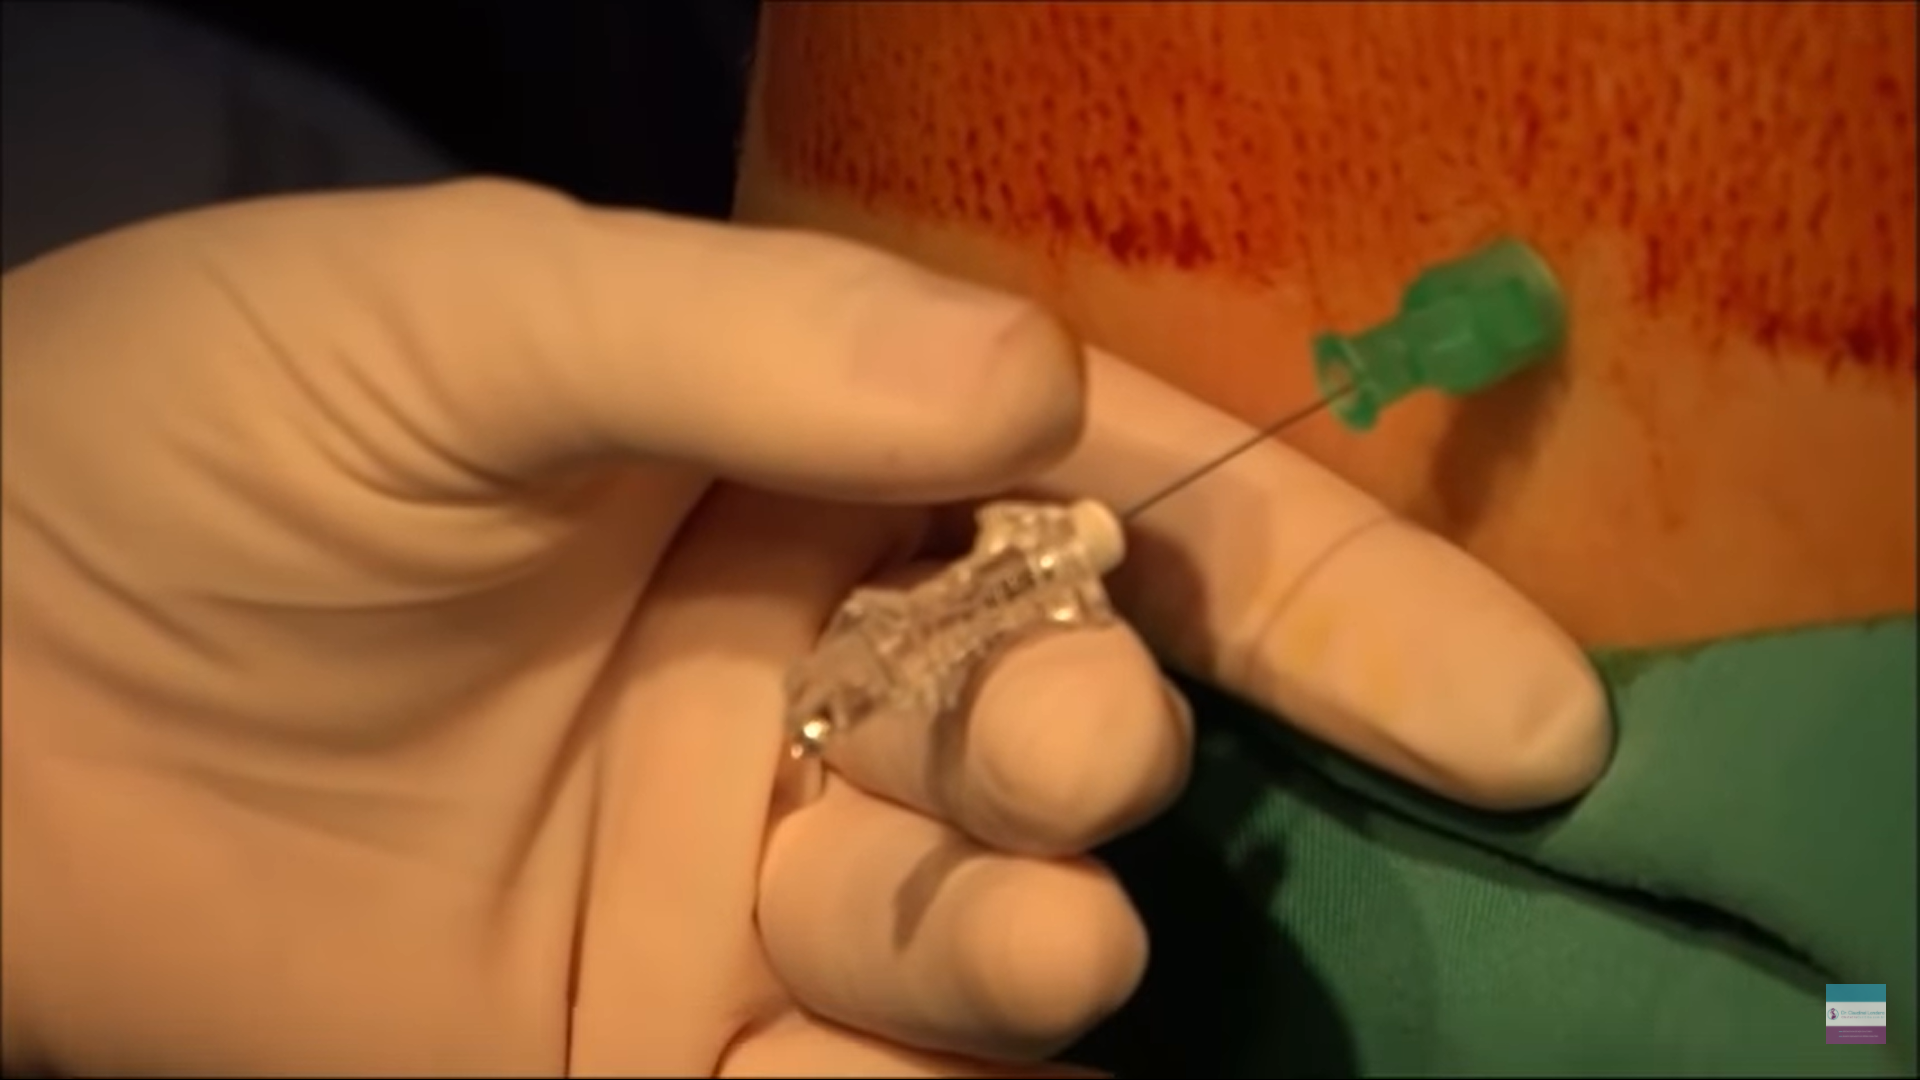
\includegraphics[width=0.6\linewidth]{capitulos/figuras/3.GotejamentoLiquor.png}
   \caption{Gotejamento do \textit{líquor}, indicação do local correto para a raquianestesia \cite{Londero2018}.}
   \label{fig:gotejamentoLiquor}
\end{figure}

A principal abordagem de treinamento para técnicas de anestesia envolve a observação da aplicação das técnicas por anestesistas experientes. Estes orientam verbalmente os aprendizes conforme cada um dos passos é executado. Adicionalmente a isto são usados: desenhos 2D, cadáveres para demonstração do procedimento, apresentação de vídeos de procedimentos, visualização 3D e técnicas de simulação. No que diz respeito ao treinamento das sensações táteis além do treinamento em cadáveres alguns simuladores fazem uso de bonecos com tecidos artificiais \textit{phantoms} que simulam pacientes \cite{Dreifaldt2006}. Um ponto negativo importante no uso de \textit{phantoms} e de cadáveres, talvez o principal, é a baixa representatividade no que diz respeito a reprodução da situação real, pois estes oferecem uma baixa variabilidade de cenários (pacientes) para treinamento.  Outro aspecto relevante no uso de \textit{phantoms} é a necessidade de reposição de peças que se desgastam com o uso e podem ter custos altos. Estes são alguns dos motivos para que em diversos hospitais a primeira experiência do anestesista em treinamento seja efetuada diretamente em um paciente \cite{Aggarwal2009, Grantcharov2008, Smith2005, Watterson2007}. Esta prática, apesar de ser efetuada sob supervisão direta de médicos experientes, traz riscos para estes pacientes e possíveis inseguranças aos aprendizes \cite{Elmofty2017}. 

O uso de simuladores para adquirir certo grau de habilidade antes de iniciar o procedimento em pacientes minimiza os riscos tanto para o aprendiz quanto para o paciente \cite{Coles2011, Akhtar2014}. A existência de diversos cenários em simuladores como os que usam \acrfull{RV} padroniza o ensino e possibilita ao aprendiz ter experiência com situações mais variadas assim como aumenta a segurança dos alunos e possibilita que a avaliação do desempenho destes seja feita de forma automatizada \cite{Willis2014}. Estes simuladores com frequência usam diferentes níveis variando as dificuldades \cite{Ullrich2012}. Permitem a redução ou eliminação de custos de manutenção de equipamentos e laboratórios físicos (3,10). 
Esta variabilidade de cenários dificilmente aconteceria na vida real em centros onde o ensino é feito diretamente em pacientes \cite{Udani2015}. Diversos simuladores utilizam dispositivos de força háptica (\textit{force feedback}) para auxiliar o aprendiz a experimentar fisicamente as sensações de resistência modeladas para os tecidos ao praticar procedimentos médicos. Este tipo de abordagem é usada em procedimentos médicos de um modo geral \cite{Escobar-Castillejos2016} assim como no caso mais específico dos procedimentos de anestesia \cite{Vaughan2013}. Existem inúmeras outras formas de como o uso de ferramentas computacionais podem auxiliar no campo da anestesia. Um exemplo é no controle automatizado de quanto anestésico aplicar a partir de respostas de medições dos níveis de consciência do paciente \cite{Mendez2009}.

\textcite{Correa2019}, na sua análise do estado da arte, relataram que as avaliações da percepção humana são pouco exploradas no campo da interação háptica para treinamento de inserção de agulhas. Eles também citam a predominância de testes subjetivos para validação das soluções propostas por parte dos usuários. Alguns trabalhos fazem uso de análises subjetivas usando gráfico de profundidade da agulha versus tempo como em \textcite{Magill2010}. Nesta tese utilizamos gráficos de força \textit{versus} deslocamento da agulha para descrever o comportamento durante a perfuração das camadas nos experimentos. Usamos também os questionários onde procuramos reduzir a subjetividade da interpretação dos gráficos. \textcite{N.2013} descreveu um simulador sofisticado porém sem avaliação do usuário. Já um outro simulador comercial foi testado por 45 anestesistas apresentando um bom \textit{feedback} sobre a qualidade da simulação em muitos aspectos. No entanto, este simulador carecia de realismo nas questões relativas ao ponto de entrada e ângulo correto de inserção da agulha \cite{Lee2012}, que são elementos críticos no procedimento real. O ponto de entrada da agulha também estava fora do escopo de um simulador acoplado a um cilindro pneumático. Este simulador foi testado por oito usuários (dois experientes e seis novatos), com foco na avaliação das habilidades do usuário através do simulador ao invés da validação do simulador em si \cite{Senac2019}. \cite{Farber2009} avaliaram ao mesmo tempo os usuários e o simulador. Os usuários foram avaliados em termos da perfuração feita por eles com relação ao tempo, caminho ótimo e atingimento de estruturas classificadas como de risco. O simulador foi avaliado a partir da resposta dos usuários a um questionário de usabilidade. Outro estudo testou o uso de um manequim de baixo custo impresso em impressora 3D contra um simulador comercial com resultados comparáveis (teste subjetivo). No entanto, este modelo carece de variabilidade, pois simula apenas um modelo de corpo para cada manequim impresso \cite{Mashari2018}. Assim, para construir critérios mais objetivos, nesta tese focamos nossos experimentos em fazer perguntas com respostas esperadas em vez de questionários para validar as opiniões dos usuários. As respostas indicam se um comportamento específico pode ser mapeado corretamente.

A apresentação de cenários de treinamento virtuais que simulam a possibilidade de visualização e sentimentos táteis que são vivenciados no procedimento real aproxima a prática de treino virtual da posterior prática em pacientes reais possibilitando um maior sentimento de segurança por parte dos anestesistas aprendizes. A aplicação de transparência em camadas pode ser utilizada num ambiente virtual permitindo a visão do interior do corpo o que pode facilitar o entendimento do aprendiz no que diz respeito a teoria do procedimento. Esta conexão da teoria com a prática é um grande trunfo no uso da \acrfull{RV} em simuladores para treinamento. Neste caso, o realismo na apresentação dos elementos envolvidos no treinamento tem um importante papel. Seja a representação 3D da agulha, do corpo ou as camadas internas que possam ser visualizadas. 

\section{Objetivos}
\label{sec:objetivos}

Esta tese tem o seguinte objetivo geral:

Desenvolver um ambiente de treinamento no que se refere às técnicas de anestesia raquidiana buscando prover um aprendizado padronizado e mais completo dos anestesistas sem incorrer em risco para os pacientes. Este treinamento será padronizado no sentido das técnicas que precisarão ser dominadas pelos usuários treinados  porém o sistema irá fazer com que os usuários que demonstrarem melhor desenvoltura nas etapas iniciais pulem etapas de demonstração de habilidades já identificadas. 

\section{Contribuições da Tese}
\label{sec:contribuicoes}

As contribuições deste trabalho envolvem a reprodução virtual das principais sensações hápticas necessárias para simular a anestesia raquidiana. Outra contribuição foi a construção de um modelo 3D real da parte lombar do corpo de uma gestante (tecidos entre a pele a cauda equina) de forma facilmente modificável via programação. Esta é uma etapa fundamental para tornar a simulação mais real e adaptável a vários cenários de testes. A variação dos tamanhos das principais camadas do modelo foi alimentada por um equação genérica criada e detalhada neste trabalho.

\section{Estrutura da Tese}
\label{sec:estrutura}

O restante do texto está estruturado da seguinte forma. O Capítulo~\ref{cap:cap2} comenta os principais conceitos e tecnologias envolvidas no desenvolvimento do ambiente de treinamento proposto.

O Capítulo~\ref{cap:cap3} contém os trabalhos relacionados a esta tese assim como o posicionamento deste trabalho frente aos demais.
No Capítulo~\ref{cap:cap4} é apresentada a proposta de trabalho que foi desenvolvida durante esta tese. 
O Capítulo~\ref{cap:cap5} apresenta os experimentos que foram feitos e uma avaliação destes em relação aos seus resultados.
Por fim, o Capítulo~\ref{cap:cap6} conclui o trabalho, apresentando as conclusões, realçando as contribuições desta tese e apontando os  trabalhos futuros.


